%% template by by Michael Shell
%% See: 
%% http://www.michaelshell.org/
%% for current contact information.
%%
%% This is a skeleton file demonstrating the advanced use of IEEEtran.cls
%% (requires IEEEtran.cls version 1.8b or later) with an IEEE Computer
%% Society journal paper.
%%
%% Support sites:
%% http://www.michaelshell.org/tex/ieeetran/
%% http://www.ctan.org/pkg/ieeetran
%% and
%% http://www.ieee.org/

%%*************************************************************************
%% Legal Notice:
%% This code is offered as-is without any warranty either expressed or
%% implied; without even the implied warranty of MERCHANTABILITY or
%% FITNESS FOR A PARTICULAR PURPOSE! 
%% User assumes all risk.
%% In no event shall the IEEE or any contributor to this code be liable for
%% any damages or losses, including, but not limited to, incidental,
%% consequential, or any other damages, resulting from the use or misuse
%% of any information contained here.
%%
%% All comments are the opinions of their respective authors and are not
%% necessarily endorsed by the IEEE.
%%
%% This work is distributed under the LaTeX Project Public License (LPPL)
%% ( http://www.latex-project.org/ ) version 1.3, and may be freely used,
%% distributed and modified. A copy of the LPPL, version 1.3, is included
%% in the base LaTeX documentation of all distributions of LaTeX released
%% 2003/12/01 or later.
%% Retain all contribution notices and credits.
%% ** Modified files should be clearly indicated as such, including  **
%% ** renaming them and changing author support contact information. **
%%*************************************************************************

\documentclass[10pt,journal,compsoc]{IEEEtran}
\usepackage{booktabs} % required for tables
\usepackage[T1]{fontenc} % Output font encoding for international characters
\usepackage{siunitx}
\usepackage{amsmath}
\usepackage{graphicx}
\usepackage{caption}
\usepackage{hyperref}

\ifCLASSOPTIONcompsoc
  % The IEEE Computer Society needs nocompress option
  % requires cite.sty v4.0 or later (November 2003)
  \usepackage[nocompress]{cite}
\else
  % normal IEEE
  \usepackage{cite}
\fi
% \usepackage[backend=bibtex,style=authoryear,natbib=true]{biblatex} % Use the bibtex backend with the authoryear citation style (which resembles APA)

% \addbibresource{main.bib} % The filename of the bibliography

\newcommand\MYhyperrefoptions{bookmarks=true,bookmarksnumbered=true,
pdfpagemode={UseOutlines},plainpages=false,pdfpagelabels=true,
colorlinks=true,linkcolor={black},citecolor={black},urlcolor={black},
pdftitle={TDoA_project_report},
pdfsubject={TDoA trajectory reconstruction},
pdfauthor={Morhunenko Mykola},
pdfkeywords={TDoA}}

% correct bad hyphenation here
\hyphenation{}

\begin{document}

\title{TDoA trajectory reconstruction}
\author{Morhunenko Mykola}
% make the title area
\maketitle

% =================================================================================
\IEEEraisesectionheading{\section{Introduction}\label{sec:introduction}}
Within the subject "Diagnostics and testing" there is a compulsory semester project for each student on a chosen topic.
The project "Time-Difference-of-Arrival (TDoA) trajectory reconstruction" sounded like the most algorithmic among other. 
The main goal is to find a trajectory of a moving object (tag) repeatedly transmitting a signal, using a set of given fixed-position receivers (anchors)
The main principal behind the TDoA trajectory reconstruction methods consists of two main phases: time synchronisation and location position estimation.
In this report both topics will be covered.
The main goal of this project is to implement in Python some algorithm for the trajectory reconstruction of a moving object from the given dataset.

% =================================================================================
\section{Problem description}
\label{sec:problem}

% =================================================================================
\section{Data description}
\label{sec:data_desc}
\begin{figure}[ht]
    \centering
    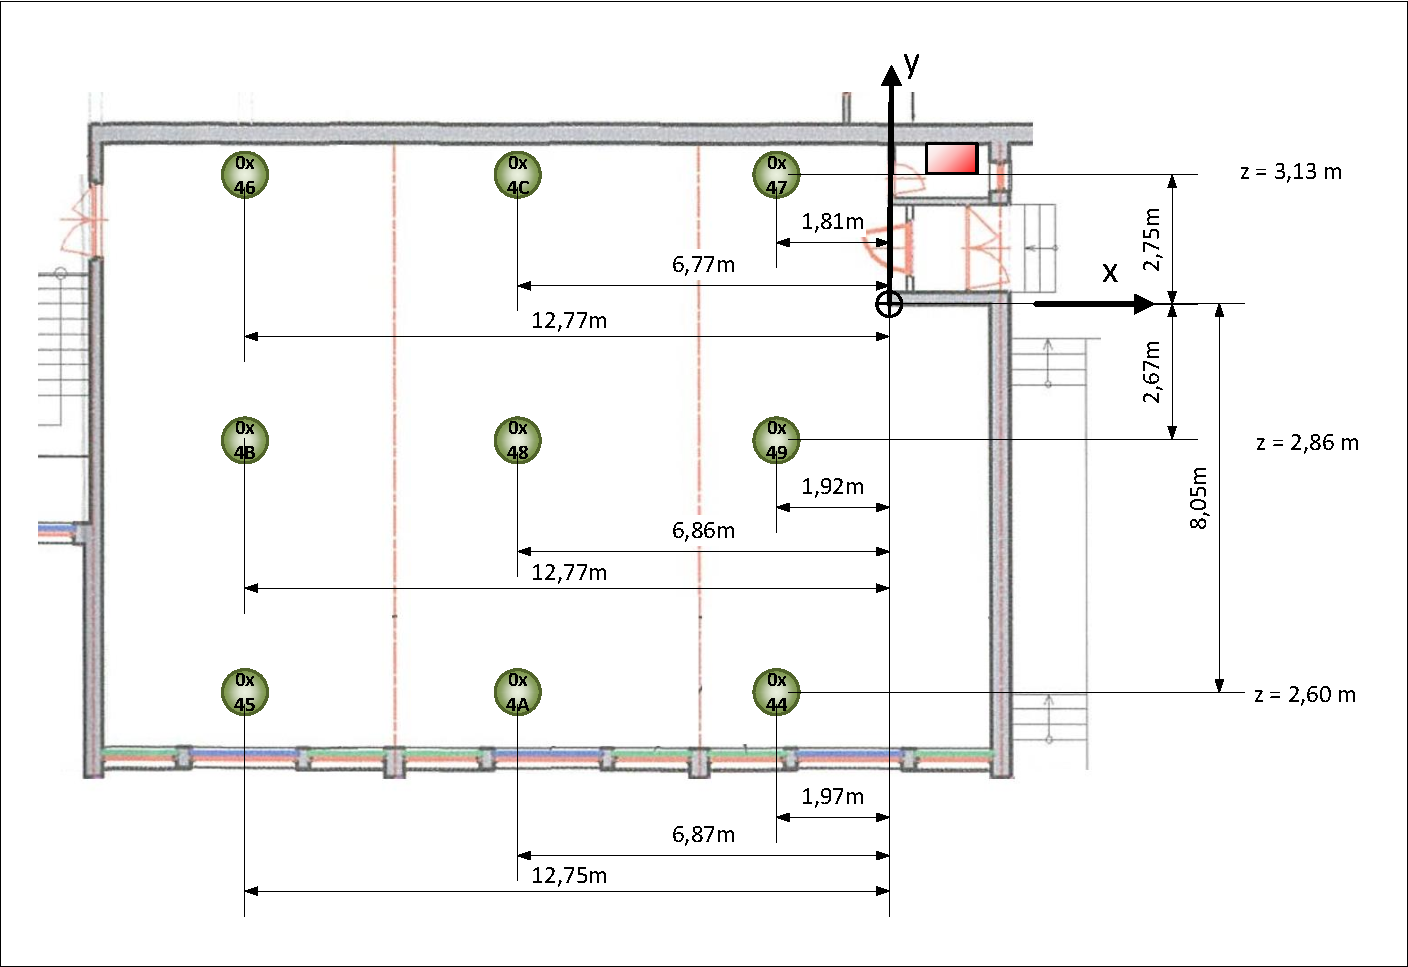
\includegraphics[width=0.48\textwidth]{graphics/UWB_map.pdf}
    \caption{The indoor map of the anchors is shown in the image. Nine anchors with hexadecimal identifiers located in a form of 3x3 grid, each row on a different height.}
    \label{fig:UWB_map}
\end{figure}
\begin{figure}[ht]
    \centering
    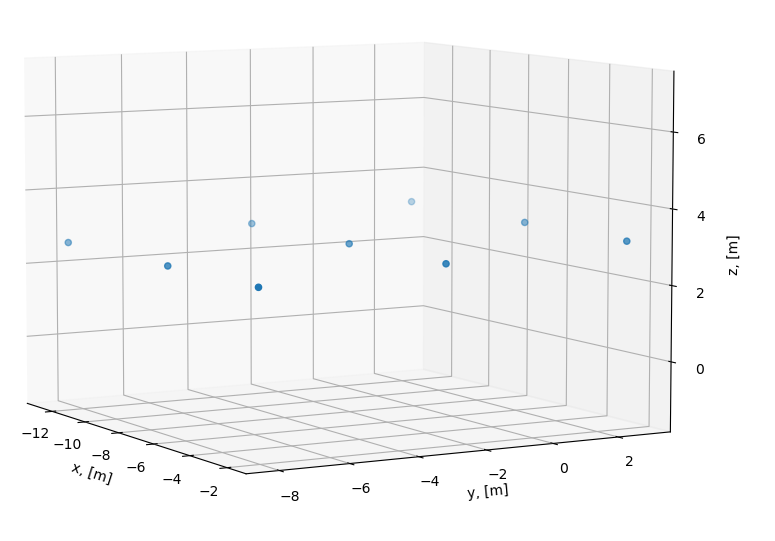
\includegraphics[width=0.48\textwidth]{graphics/room3D.png}
    \caption{The indoor map of the anchors in 3D.}
    \label{fig:3D_map}
\end{figure}

Along with the project assignment, two files from the real-world experiments, indoor map (see \autoref{fig:UWB_map}) were provided. So the room in 3D can be visualized as in \autoref{fig:3D_map}.

For each experiment, there are "blinks" and "syncs" files.
"syncs.csv" file contains synchronisation messages between anchors in a form "addr\_tx, addr\_rx, ts\_tx, ts\_rx, timestamp",  where first two columns are addresses of transmitter and receiver respectively, next two columns corresponds to timestamps of a recording module DWM1000 on each anchor, which measures time in it's own units (here and further - $[\SI{}{dw}]$) where $\SI{1}{dw} = \frac{1}{(128*499,2*10^6)}\SI{}{s}$. 
The last column corresponds to the timestamp of an experiment recording system, which runs on Unix, time in $[\SI{}{ms}]$.
"blinks.csv" file contains location messages between an unknown moving object and anchors in a format "addr\_tx, addr\_rx, ts\_rx, ts\_tx, id" where first two columns addresses of transmitter and receiver respectively, next two columns are corresponding timestamps of a message transmission and receiving, and the last column corresponds to the message id.

The 

% =================================================================================
\section{Related works}
\label{sec:ps}
The TDoA indoor localisation is quite old and well-described topic. For example in \cite{Yuzan2019} there is a proposed method for an online time-synchronisation and trajectory reconstruction. The general method is well-described in a \cite{Keefe2017}.

% =================================================================================
\section{Chosen method}
\label{sec:method}

\subsection{Trajectory reconstruction}
\label{sec:traj_recon}
Here and further consider already synchronised time with respect to the main anchor.
The iterative location estimation using the TDoA was used in the trajectory reconstruction step.
Let any two non similar anchors to be $i$ and $j$ located on a distance $d_{ij}$.
Timestamps of received signals from the tag by each anchor are denoted as $t_i$ and $t_j$.
Time difference of arrival of two signal is
\begin{equation}
    \Delta{t} = |t_j - t_i|.
    \label{eq:dt1}
\end{equation}
From another side, let us consider the coordinates of a moving object as $(x, y, z)$, coordinates of two anchors as $(x_i, y_i, z_i)$ and $(x_j, y_j, z_j)$ respectively.
The distance from a tag to each anchor can be written as
\begin{equation}
    d_i = \sqrt{(x-x_i)^2 + (y-y_i)^2 + (z - z_i)^2}.
    \label{eq:dist}
\end{equation}
Considering the time-velocity relation (distance = velocity * time) 
\begin{equation}
    \Delta{d} = c\Delta{t},
\end{equation}
and the equation \eqref{eq:dt1}, let us define the function f:
\begin{equation}
    \label{eq:f}
    f = |d_j - d_i| - c |t_j - t_i| = 0.
\end{equation}
Where both $t_j$ and $t_i$ are given, $c$ is a speed of a signal (speed of light) and $d_i, d_j$ together contain 3 unknowns. 
To find them, at least 3 such equations are needed, which corresponds to at least 3 anchors.
This problem is already formulated as a non-linear least squares (NLLS) problem, so it can be solved with any optimizer for such a task.

The gradient of $f$ needed for NLLS can be computed as:
\begin{equation}
    \nabla f(\left.x, y, z\right)=\left[\begin{array}{c}
    \dfrac{\partial f}{\partial x}\\
    \dfrac{\partial f}{\partial y}\\
    \dfrac{\partial f}{\partial z}
    \end{array}\right] = \left[\begin{array}{c}
    \frac{(\frac{x-x_j}{d_j} - \frac{x-x_i}{d_i})(d_j - d_i)}{|d_j - d_i|}\\
    \frac{(\frac{y-y_j}{d_j} - \frac{y-y_i}{d_i})(d_j - d_i)}{|d_j - d_i|}\\
    \frac{(\frac{z-z_j}{d_j} - \frac{z-z_i}{d_i})(d_j - d_i)}{|d_j - d_i|}
    \end{array}\right].
\end{equation}

\subsection{Time synchronisation}
\label{sec:time_sync}
The custom approach was chosen for the time synchronization as far as the found methods were too complicated to implement. 
Let $T_{ij}$ be the time of flight from anchor $i$ to $j$, the main anchor index to be $m$.
If clocks on two anchors are perfectly synchronized, the ideal timestamps of sending a message from $t_m$ to $t_i$ would be:
\begin{equation}
    \label{eq:sync_ideal}
    t_{i}^* = t_m + T_{mi},
\end{equation}
but in the real world, this time would be
\begin{equation}
    \label{eq:sync}
    t_{i}^{'} = t_m + T_{mi} + e_{mi},
\end{equation}
where $e_{mi}$ stands for some error. 

The relation of the number of sync messages to blink messages in given files is about $\frac{18}{1}$. 
More scientifically, anchors are synchronized at about $\SI{13.9}{Hz}$, but messages from moving objects don't really have a fixed frequency, the difference in time between messages varies.
Under the assumption that the time shift between two clocks will not change a lot between sync messages, because they are much more frequent than blink messages, the following synchronization approach is proposed.
The array $A_{cor}$ contains time corrections for each anchor with respect to the main anchor. 
Continuing analysing equations \eqref{eq:sync_ideal} and \eqref{eq:sync}, the time correction in case the message was sent from the main anchor can be found as
\begin{equation}
    t_{c} = t_i^{'} - t_i^{*} = A_{cor}[i]
\end{equation}
and the matrix $A_{cor}$ can be updated.

The same if the sync message was transferred from any $t_i$ to $t_m$, the time correction can be found as
\begin{equation}
    t_i^{*} = t_m - T_{im},
\end{equation}
\begin{equation}
    t_i^{'} = t_m - T_{im} + e_{im},
\end{equation}
\begin{equation}
    A_{corr}[i] = t_i^{'} - t_i^{*},
\end{equation}
then at any time $t \approx t_i$ can be transformed to the main anchors' time domain $t^m$ as
\begin{equation}
    t_i^{m} = t_i + A_{corr}[i].
\end{equation}

As far as not all anchors receive every synchronisation signal, the matrix $A_{cor}$ updating can be accelerated consider pairwise messages between any two anchors $i$ and $j$, the sync message going from $i \rightarrow j$. If the anchor $i$ is not yet synchronised with the network, we can update only it. In the main anchor time domain it is as following:
\begin{equation}
    t_i^{*} = t_j + A_{cor}[j] - T_{ij},
\end{equation}
\begin{equation}
    t_i^{'} = t_j + A_{cor}[j] - T_{ij} + err_{ij},
\end{equation}
\begin{equation}
    A_{cor}[i] = t_i^{'} - t_i^{*}.
\end{equation}

In the opposite situation, when the anchor $j$ is not yet synchronised,
\begin{equation}
    t_j^{*} = t_i + A_{cor}[i] + T_{ij},
\end{equation}
\begin{equation}
    t_j^{'} = t_i + A_{cor}[i] + T_{ij} + err_{ij},
\end{equation}
\begin{equation}
    A_{cor}[j] = t_j^{'} - t_j^{*}.
\end{equation}

% =================================================================================
\section{Implementation}
\label{sec:impl}

% =================================================================================
\section{Error measurement}
\label{sec:error}

% =================================================================================
\section{Conclusion}
The conclusion goes here.

% =================================================================================
\bibliography{main}{}
\bibliographystyle{ieeetr}
\cleardoublepage

\end{document}

